% This is the Reed College LaTeX thesis template. Most of the work
% for the document class was done by Sam Noble (SN), as well as this
% template. Later comments etc. by Ben Salzberg (BTS). Additional
% restructuring and APA support by Jess Youngberg (JY).
% Your comments and suggestions are more than welcome; please email
% them to cus@reed.edu
%
% See http://web.reed.edu/cis/help/latex.html for help. There are a
% great bunch of help pages there, with notes on
% getting started, bibtex, etc. Go there and read it if you're not
% already familiar with LaTeX.
%
% Any line that starts with a percent symbol is a comment.
% They won't show up in the document, and are useful for notes
% to yourself and explaining commands.
% Commenting also removes a line from the document;
% very handy for troubleshooting problems. -BTS

% As far as I know, this follows the requirements laid out in
% the 2002-2003 Senior Handbook. Ask a librarian to check the
% document before binding. -SN

%%
%% Preamble
%%
% \documentclass{<something>} must begin each LaTeX document
\documentclass[12pt,twoside]{ugathesis}
% Packages are extensions to the basic LaTeX functions. Whatever you
% want to typeset, there is probably a package out there for it.
% Chemistry (chemtex), screenplays, you name it.
% Check out CTAN to see: http://www.ctan.org/
%%
\usepackage{graphicx,latexsym}
\usepackage[french]{babel}
\usepackage{amsmath}
\usepackage{amssymb,amsthm}
\usepackage[dvipsnames]{xcolor} % tk: for more color
\usepackage{xcolor}
\usepackage{eso-pic}
\usepackage{longtable,booktabs,setspace}
\usepackage{chemarr} %% Useful for one reaction arrow, useless if you're not a chem major
\usepackage[hyphens]{url}
\usepackage{pdfpages}
\usepackage{tikz}
\usetikzlibrary{calc}
% Added by CII
\usepackage{hyperref}
\usepackage{lmodern}
\usepackage{float}
\floatplacement{figure}{H}
% End of CII addition
\usepackage{rotating}
\usepackage{upgreek} % tk : pour pouvoir utiliser le symbole µ droit (pas en itallic)
\usepackage{pdfpages} % tk : pour pouvoir insérer des fichiers pdf dans le corp de texte
\usepackage{lscape} % tk : pour pouvoir insérer des images au format paysage
\newcommand{\blandscape}{\begin{landscape}}
\newcommand{\elandscape}{\end{landscape}}
\usepackage[utf8]{inputenc}

% Next line commented out by CII
%%% \usepackage{natbib}
% Comment out the natbib line above and uncomment the following two lines to use the new
% biblatex-chicago style, for Chicago A. Also make some changes at the end where the
% bibliography is included.
%\usepackage{biblatex-chicago}
%\bibliography{thesis}


% Added by CII (Thanks, Hadley!)
% Use ref for internal links
\renewcommand{\hyperref}[2][???]{\autoref{#1}}
\def\chapterautorefname{Chapter}
\def\sectionautorefname{Section}
\def\subsectionautorefname{Subsection}
% End of CII addition

% Added by CII
\usepackage{caption}
\captionsetup{width=5in}
% End of CII addition

% \usepackage{times} % other fonts are available like times, bookman, charter, palatino


% To pass between YAML and LaTeX the dollar signs are added by CII
\title{THÈSE}
\author{Thomas Karaouzene}
\lab{Techniques de l'Ingénierie Médicale et de la Complexité - Informatique,
Mathématiques et Applications de Grenoble (TIMC-IMAG)}
\date{07 novembre 2017}
\division{Mathematics and Natural Sciences}
\advisor{Pierre Ray}
%If you have two advisors for some reason, you can use the following
% Uncommented out by CII
\altadvisor{Nicolas Thierry-Mieg}
% End of CII addition
%\institution{}
%\degree{}

%%% Remember to use the correct department!
\department{Ingénierie de la Santé, de la Cognition et Environnement (EDISCE)}
% if you're writing a thesis in an interdisciplinary major,
% uncomment the line below and change the text as appropriate.
% check the Senior Handbook if unsure.
%\thedivisionof{The Established Interdisciplinary Committee for}
% if you want the approval page to say "Approved for the Committee",
% uncomment the next line
%\approvedforthe{Committee}

% Added by CII
%%% Copied from knitr
%% maxwidth is the original width if it's less than linewidth
%% otherwise use linewidth (to make sure the graphics do not exceed the margin)
\makeatletter
\def\maxwidth{ %
  \ifdim\Gin@nat@width>\linewidth
    \linewidth
  \else
    \Gin@nat@width
  \fi
}
\makeatother

\renewcommand{\contentsname}{Table of Contents}
% End of CII addition

\setlength{\parskip}{0pt}

% Added by CII
  %\setlength{\parskip}{\baselineskip}
  \usepackage[parfill]{parskip}

\providecommand{\tightlist}{%
  \setlength{\itemsep}{0pt}\setlength{\parskip}{0pt}}

\Acknowledgements{

}

\Dedication{

}

\Preface{

}

\Abstract{

}

	\usepackage{tikz}
% End of CII addition
%%
%% End Preamble
%%
%

\begin{document}

% Everything below added by CII
  \maketitle

\frontmatter % this stuff will be roman-numbered
\pagestyle{empty} % this removes page numbers from the frontmatter



  \hypersetup{linkcolor=black}
  \setcounter{tocdepth}{3}
  \tableofcontents

  \listoftables

  \listoffigures



\mainmatter % here the regular arabic numbering starts
\pagestyle{fancyplain} % turns page numbering back on

\chapter{thesisdown::thesis\_epub:
default}\label{thesisdownthesis_epub-default}

\chapter*{Résumé}\label{resume}
\addcontentsline{toc}{chapter}{Résumé}

\chapter{Introduction}\label{introInf}

\chapter{Investigation génétique et physiologique de la
globozoospermie}\label{globo}

\section{Introduction sur la
globozoospermie}\label{introduction-sur-la-globozoospermie}

Comme expliqué précédemment, La globozoospermie est un phénotype rare
(\textless{} 0.1\% des patients infertiles) mais néanmoins sévère
{[}\protect\hyperlink{ref-Sen2009}{1}{]} de teratozoospermie menant à
l'infertilité masculine. Cette anomalie est caractérisée par la présence
de spermatozoïdes présentant une tête ronde dépourvue d'acrosome et
d'une pièce intermédiaire désorganisée dans l'éjaculat
{[}\protect\hyperlink{ref-Singh}{2},
\protect\hyperlink{ref-Pedersen1974}{3}{]} (\textbf{Figure :
}\ref{fig:pictglobospz}). En plus des anomalies morphologiques, les
spermatozoïdes globozoocéphales présentent également des
désorganisations au niveau moléculaire. Par exemple, le facteur
spermatique PLC\(\zeta\) requit pour l'activation ovocytaire, est absent
ou en quantité infime dans les spermatozoïdes globozoocéphales
{[}\protect\hyperlink{ref-Heytens2009}{4}--\protect\hyperlink{ref-Yoon2008}{6}{]}
compromettant ainsi l'activation ovocytaire et expliquant le faible taux
de fécondation observés en fécondation \emph{in vitro} (IVF) et en ICSI
(intra cytoplasmic sperm injection)
{[}\protect\hyperlink{ref-Dam2006}{7}{]}. On distingue la
globozoospermie totale avec 100\% des spermatozoïdes présentant le
phénotype ou partielle en fonction du taux de spermatozoïdes atteints.
Bien que l'infertilité masculine soit souvent la résultante de plusieurs
facteurs, les premières études présentant des patients atteints par un
phénotype complet {[}\protect\hyperlink{ref-Sen2009}{1}{]} suggéraient
que la globozoospermie était une exception. De plus les caractéristiques
morphologiques très typiques des spermatozoïdes laissaient penser à une
cause monogénique. En 2007, une étude portant sur une famille juive
ashkénaze comprenant six frères dont trois atteins a pu lier ce
phénotype à une mutation homozygotes sur le gène \emph{SPATA16} présente
chez les trois frères atteint {[}\protect\hyperlink{ref-Dam2007}{8}{]}.
Cependant, dans la même étude, 29 autres patients présentant le même
phénotype ont été analysés, et pour ceux-ci, aucun variant du gène
\emph{SPATA16} n'a pu être lié au phénotype
{[}\protect\hyperlink{ref-Dam2007}{8}{]} indiquant clairement que les
mutations de ce gène n'étaient pas les seules responsables. En 2011, une
autre étude portant sur une cohorte de 20 patients Tunisiens a pu mettre
en évidence une délétion homozygote de 200kb emportant la totalité du
gène \emph{DPY19L2} chez 15 des 20 patients analysés
{[}\protect\hyperlink{ref-Harbuz2011}{9}{]}. Les études effectuées
ultérieurement sur ce phénotype ont ensuite pu montrer que les
altérations du gène \emph{DPY19L2}, et notamment cette délétion, étaient
responsables de la majorité des cas de globozoospermie
{[}\protect\hyperlink{ref-Ray2011}{10},
\protect\hyperlink{ref-ElInati2012}{11}{]}.

\begin{figure}

{\centering 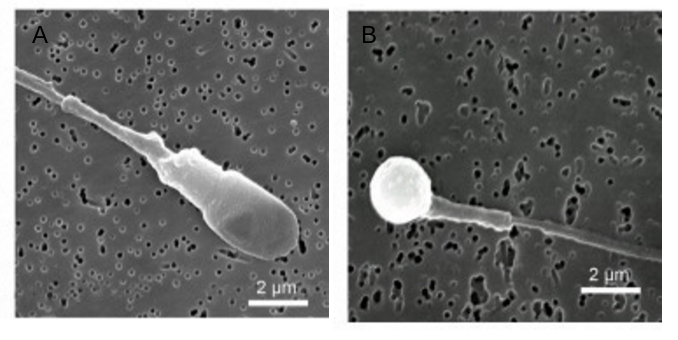
\includegraphics[scale=0.6]{figure/globo_normal_spz} 

}

\caption[Observation au microscope à balayage de spermatozoïdes]{\textbf{\emph{Observation au microscope à balayage de
spermatozoïdes}. Adapté d'après
{[}\protect\hyperlink{ref-Harbuz2011}{9}{]}} : \textbf{A} :
Spermatozoïde normal. \textbf{B} : Spermatozoïde globozoocéphale. TODO
:: changer les photos avec celles sur lesquelles on voit l'acrosome
colorés)}\label{fig:pictglobospz}
\end{figure}








En 2012, le développement d'un modèle murin KO \emph{Dpy19l2}\(^{-/-}\)
a permis de mieux comprendre les mécanismes moléculaires impliqués dans
la globozoospermie causée par la délétion du gène \emph{DPY19L2} chez
l'humain {[}\protect\hyperlink{ref-Pierre2012}{12}{]}. Ce modèle de
souris KO présentant les mêmes caractéristiques que les patients humains
; Tout d'abord, ces souris étaient infertiles et présentaient des
spermatozoïdes globozoocéphales (\textbf{Figure :
}\ref{fig:pictmouseglobo}) mais aussi et surtout, l'ensembles des autres
dysfonctionnements étaient retrouvés, c'est à dire : l'absence de
l'acrosome, les défauts morphologiques du noyau, de l'enveloppe
nucléaire et de l'acroplaxome ainsi que le mauvais positionnement de la
manchette {[}\protect\hyperlink{ref-Pierre2012}{12}{]}. Ainsi il a pu
être démontré que la protéine Dpy19l2 étaient principalement exprimée
dans le spermatide et plus spécifiquement dans la membrane nucléaire
interne faisant face à la vésicule acrosomale et que l'absence de cette
protéine entrainait la déstabilisation à la fois de la lamine nucléaire,
de la jonction entre l'acroplaxome et l'enveloppe nucléaire
{[}\protect\hyperlink{ref-Pierre2012}{12}{]}.

\newpage 

\begin{figure}

{\centering 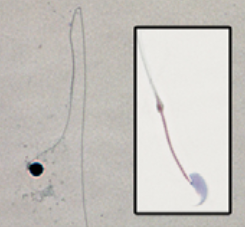
\includegraphics[scale=0.8]{figure/mouse_globo_spz} 

}

\caption[Comparaison entre les spermatozoïdes des souris *Dpy19l2*$^{-/-}$ (à gauche) et les souris sauvages *Dpy19l2*$^{+/+}$ (à droite)]{\textbf{\emph{Comparaison entre les spermatozoïdes
des souris \emph{Dpy19l2}\(^{-/-}\) (à gauche) et les souris sauvages
\emph{Dpy19l2}\(^{+/+}\) (à droite)}. D'après
{[}\protect\hyperlink{ref-Pierre2012}{12}{]}}.}\label{fig:pictmouseglobo}
\end{figure}






\newpage

\section{\texorpdfstring{Résultats 1 : Les mécanismes mutationnels
entrainant la délétion au locus de \emph{DPY19L2} chez
l'humain}{Résultats 1 : Les mécanismes mutationnels entrainant la délétion au locus de DPY19L2 chez l'humain}}\label{mecamut}

\subsection{Article n° 1:}\label{article-n-1}

\textbf{Fine Characterisation of a Recombination Hotspot at the
\emph{DPY19L2} Locus and Resolution of the Paradoxical Excess of
Duplications over Deletions in the General Population}

Coutton C, Abada F, \textbf{Karaouzène T}, Sanlaville D, Satre V,
Lunardi J, Jouk PS, Arnoult C, Thierry-Mieg N, Ray PF

\textsuperscript{*} Co-premiers auteurs

PLOS GeneticS, Mars 2013

\newpage

\subsubsection{Contexte et objectifs}\label{contexte-et-objectifs}

Chez les mammifères il existe trois paralogues de \emph{DPY19L2} de
fonctions encore inconnues et un pseudogène présentant une très forte
homologie de séquence (\textgreater{} 95\%)
{[}\protect\hyperlink{ref-Carson2006}{13}{]}. Chez l'Homme, ce gène est
flanqué de deux séquences présentant une forte homologie
(\textgreater{}95\%) d'une taille de 28kb. Ces séquences appelées LCRs
(\emph{low copy repeats}) représentent une large portion du génome
humain {[}\protect\hyperlink{ref-Cheung2003}{14},
\protect\hyperlink{ref-Bailey2002}{15}{]} et vont, de par leur homologie
favoriser les duplications de gènes jouant ainsi un rôle important dans
l'évolution des génomes des vertébrés
{[}\protect\hyperlink{ref-Walsh2003}{16},
\protect\hyperlink{ref-Ohno1970}{17}{]}. Dans le cas de \emph{DPY19L2},
ces LCRs vont, au cours de la méiose entrainer la venue de
recombinaisons homologues non-allélique (NAHR) donnant lieu soit à une
délétion du gène \emph{DPY19L2} et la formation d'un ADN circulaire
comprenant le gène soit à un allèle possédant deux copies du gène tandis
que l'autre n'en possède aucune
{[}\protect\hyperlink{ref-Harbuz2011a}{18}{]}.

Ce mécanisme de NAHR devrait, en théorie, engendrer la formation de plus
d'allèles délétés que d'allèles dupliqués puisque les cas présentés en
figures \ref{fig:pictnahr} - \textbf{2} et \ref{fig:pictnahr} -
\textbf{3} induisent la formation d'un allèle délété tandis que seul le
cas \ref{fig:pictnahr} - \textbf{3} forme un allèle dupliqué
{[}\protect\hyperlink{ref-Liu2012}{19}{]}. Cependant, les données mises
à disposition par la base de données
\href{http://dgv.tcag.ca/dgv/app/home}{\emph{Database of Genomic
Variants}} (DGV) {[}\protect\hyperlink{ref-MacDonald2014}{20}{]}
indiquent un excès de duplication puisque sur un total de 6575 individus
analysés, 83 duplications et de 26 délétions hétérozygotes ont été
observées pour le locus de \emph{DPY19L2}.

Ainsi, dans cette étude, notre équipe a cherchée à caractériser
précisément le mécanisme génétique et les facteurs favorisant la
survenue par NAHR de la délétion homozygote récurrente emportant
totalement le gène DPY19L2. De même, nous avons tenté de résoudre le
paradoxe observé entre le modèle théorique de NAHR et la fréquence des
allèles observée dans la population générale afin de confirmer les
données fournies dans les bases de données et ainsi écarter l'hypothèse
d'un biais causé par la présence du pseudogène \emph{DPY19L2P1} très
homologue avec \emph{DPY19L2}
{[}\protect\hyperlink{ref-Carson2006}{13}{]}.

Dans ce contexte j'ai pu participer à diverses manipulations de biologie
moléculaire tel que l'extraction d'ADN spermatique, quantification des
délétions / duplications \emph{de novo}. De même, j'ai pu contribuer au
diverses analyses statistiques.

\newpage 

\begin{figure}

{\centering \includegraphics[scale=0.5]{figure/nahr_process} 

}

\caption[Représentation schématique du mécanisme de NAHR]{\textbf{\emph{Représentation schématique du mécanisme de
NAHR}. Adapté d'après {[}\protect\hyperlink{ref-Pierre2012}{12}{]}} :
Lors d'un NAHR interchromatidien, un allèle dupliqué et un allèle délété
sont formés. Lors d'un NAHR intrachrmatidien, seule un allèle délété est
produit, en même temps qu'un petit ADN circulaire qui sera éliminé par
la suite.}\label{fig:pictnahr}
\end{figure}








\newpage

\includepdf[pages=-]{bib/DPY19L2_2013}

\newpage

\subsubsection{Principaux résultats}\label{principaux-resultats}

Alors que les résultats précédents confirment un excès de l'allèle
dupliqué de \emph{DPY19L2} dans la population générale, nous avons par
la suite cherché à déterminer les fréquences de duplications / délétions
\emph{de novo} de ce même locus. Ceci ayant pour but de déterminer si
cet excès est dû à une sélection de l'allèle dupliqué ou au fait que
celui-ci était effectivement produit plus fréquemment que l'allèle
délété. Pour ce faire nous avons quantifié le taux d'apparition de ces
événements génétiques à partir d'ADN spermatique. Les spermatozoïdes
étant le produit direct de la méiose, ils sont donc les reflets
d'haplotypes produits \emph{de novo}. Pour cela, nous avons analysé par
PCR digitale l'ADN spermatique de trois donneurs ainsi que l'ADN
spermatique constitué d'un mix provenant de ces trois donneurs. Leur ADN
a tout d'abord été dilué en série de sorte à ce qu'environ 25\% des 96
puits de la PCR contiennent un événement (délétion ou duplication).
Ainsi, en acceptant qu'un génome haploïde humain représente 3pg, 50ng
d'ADN spermatique furent déposés dans chaque puit pour la PCR spécifique
à la délétion, et 100ng dans chaque puit spécifique à a duplication.
Chaque puit contient donc une partie de cette charge d'ADN initiale. La
distribution de cette charge d'ADN au sein des 96 puits peut donc
s'apparier à un tirage sans remise, la probabilité qu'un puit soit
positif pour un événement chromosomique (duplication ou délétion) peut
donc être modélisé par une loi hypergéométrique (\textbf{Équation} :
\eqref{eq:hypergeo}). Nous permettant ainsi d'estimer la fréquence
duplication / délétion \(\lambda\) pour chaque donneur
(\textbf{Équation} : \eqref{eq:lambda}).

\begin{equation} 
\frac{\frac{(N - R)!}{W!(N-R-W)!}}{\frac{N!}{W!(N-W)!}} = \frac{(N-R)!(N-W)!}{N!(N-W-R)!} = \prod_{i=0}^{R-1}{\frac{N-W-i}{N-i}}
\label{eq:hypergeo}
\end{equation}

\begin{equation} 
\lambda = \frac{R}{N}
\label{eq:lambda}
\end{equation}

Où :\\
. \(N\) : représente le nombre de copie de chromosome 12 dans la charge
d'ADN initiale (1.6x10\({^6}\) pour la PCR spécifique à la délétion,
3.2x10\({^6}\) pour la PCR spécifique à la duplication)\\
. \(W = \frac{N}{96}\) correspond au nombre de copiede chromosome 12 par
puit\\
. \(R\) représente le nombre total de recombinaison observées

L'intervalle de confiance (IC) à 95\% est ensuite calculé grâce à une
loi binomiale de sorte à modéliser la dilution initiale pour obtenir
l'ADN d'\emph{entrée}. Le puit contenant le \emph{pool} des trois ADN
spermatique est donc celui ayant les résultats les plus robustes, l'IC
étant le plus resserré et permet donc d'établir le taux de délétion
\emph{de novo} à 1.8 x 10\(^{-5}\) (IC 95\% : 1.4x 10\(^{-6}\); 2.2x
10\(^{-6}\)) tandis que le taux de duplication \emph{de novo} est estimé
à 7.7 x 10\(^{-6}\) (IC 95\% : 6.1 x 10\(^{-6}\); 9.7 x 10\(^{-6}\))
montrant un enrichissement environ deux fois supérieur des délétions par
rapport aux duplications sur le site de \emph{DPY19L2}.

Ainsi, de manière paradoxale, les délétions \emph{de novo}
apparaitraient, au cours de la méiose, deux fois plus fréquemment que
les duplications \emph{de novo} tandis que l'allèle dupliqué est trois
fois plus fréquent que l'allèle délété dans la population générale. Cet
effet pourrait en partie être due aux effets de sélection naturelle. En
effet, Bien qu'à notre connaissance, les femmes portant l'allèle délété
à l'état homozygote ne soient caractérisées par aucun phénotype, les
hommes, eux sont 100\% infertiles tandis que l'allèle dupliqué ne
subirait aucune sélection.\\
Cette étude a également été pour notre équipe l'occasion d'effectuer une
étude plus approfondie des LCRs flanquant le locus de \emph{DPY19L2}.
Pour cela, nous avons génotypé 20 SNPs spécifiques des LCRs télomériques
et centromériques. À partir de ces données, 5 points de cassures
distincts (BP1-5) ont pu être identifiés sur les 185 allèles recombinés
étudiés (108 délétés et 77 dupliqués). L'ensemble de ces points de
cassures sont localisés dans une région d'environ 1150 pb. L'analyse
bioinformatique de cette région a permis de mettre en évidence, au
centre de cette région, 13 nucléotides (CCNCCNTNNCCNC) constituant un
site de reconnaissance consensus de la protéine PRDM9. Cette protéine à
doigts de zinc étant connue pour son rôle central dans l'activation de
la transcription dans les premières phases de la prophase méiotique
ainsi que pour être à impliqué dans les mécanismes de recombinaisons
chromosomique au cours de la méiose chez l'humain et la souris
{[}\protect\hyperlink{ref-Parvanov2010}{21},
\protect\hyperlink{ref-Baudat2010}{22}{]}.

\newpage

\section{Résultat 2 : La transcriptomique}\label{transcriptome}

\subsection{Article n° 2:}\label{article-n-2}

\textbf{Comparative testicular transcriptome of wild type and
globozoospermic Dpy19l2 knock out mice}

\textbf{Karaouzène T} , El Atifi M, Issartel JP, Grepillat M, Charles
Coutton C, Martinez D, Arnoult C and Ray PF

Basic and Clinical Andrology, 2013

\newpage

\subsubsection{Contexte et objectifs}\label{contexte-et-objectifs-1}

Dans des études précédentes, notre équipe à réussit à démontrer que la
protéine DPY19L2 était localisée dans la membrane interne des noyaux des
spermatides pendant la spermatogénèse et qu'elle était nécessaire pour
fixer l'acrosome au noyau {[}TODO: insert ref{]}. De même, nous avons pu
mettre en évidence que dans des cellules HEK cette protéine colocalisait
avec la protéine SUN5 et que \emph{Dpy19l2} pourrait être un partenaire
de SUN5 {[}\protect\hyperlink{ref-Pierre2012}{12}{]}. Nous avons cherché
à observer si, comme la protéine SUN5. Chez la souris, la protéine Sun1
est elle aussi nécessaire à la gamétogenèse et est connue pour permettre
l'interaction entre le noyau et les télomères
{[}\protect\hyperlink{ref-Ding2007}{23}{]}. Dans cette étude nous avons
donc chercher à savoir si l'absence de la protéine Dpy19l2 pouvait
entrainer des dérèglement transcriptionnelle qui pourrait, entre autres,
expliquer l'absence de la protéine PLC\(\zeta\) dans les spermatozoïdes
globozoocéphales.

De plus, au cours de l'élevage des souris \emph{Dpy19l2} KO au sein de
notre laboratoire nous avons pu observer un excès de naissance de souris
mâle lorsque l'on croisait deux souris \emph{Dpy19l}\(^{+/-}\). Ainsi,
en comparant les sexes des souris obtenues lors de 6 premières
naissances (\emph{Birth 1-6}) on observe un total de 28 souris mâles
pour 16 souris femelles. La p-valeur obtenue en effectuant un test de
\(\chi^2\) comparant ces deux effectifs était égale à 0.0486272 laissant
supposé l'existence d'un réel, bien que faible, enrichissement en souris
mâles.

C'est donc afin d'expliquer l'absence de la protéine \emph{Plc}\(\zeta\)
dans les spermatozoïdes des souris \emph{Dpy19l2}\(^{-/-}\) ainsi que
l'enrichissement en souris mâle dans les naissances issues
d'accouplement de souris \emph{Dpy19l2}\(^{+/-}\) que nous avons
effectué une analyse comparative du transcriptome testiculaire de deux
souris \emph{Dpy19l2}\(^{+/+}\) (S1\textsuperscript{+} et
S2\textsuperscript{+}) et deux souris \emph{Dpy19l2}\(^{-/-}\)
(S1\textsuperscript{-} et S2\textsuperscript{-}) ayant pour but de
mettre en évidence d'éventuels dérèglements transcriptionnels chez la
souris KO.

Dans cette étude j'ai pu effectuer l'intégralité des manipulations de
biologie moléculaire tel que la mise en place du protocole de génotypage
des souris, l'extraction de l'ARN testiculaire de souris et l'analyse
sur puce, ainsi que l'intégralité de l'analyse bioinformatique des
résultats.

\newpage

\begin{figure}

{\centering \includegraphics{thesis_files/figure-latex/plotborn-1} 

}

\caption[Quantification des sexes des souris observées lors de chaque naissances issues d'un croisement de deux souris hétérozygotes *Dpy19l2*$^{+/-}$]{\textbf{\emph{Quantification des sexes des souris
observées lors de chaque naissances issues d'un croisement de deux
souris hétérozygotes \emph{Dpy19l2}\(^{+/-}\)}} : Après 6 naissances, 16
souriceaux mâles sont nés pour seulement 28 femelles, ainsi le test du
\(\chi^2\) comparant ces valeurs donne une p-valeur de 0.0486272.}\label{fig:plotborn}
\end{figure}







\newpage

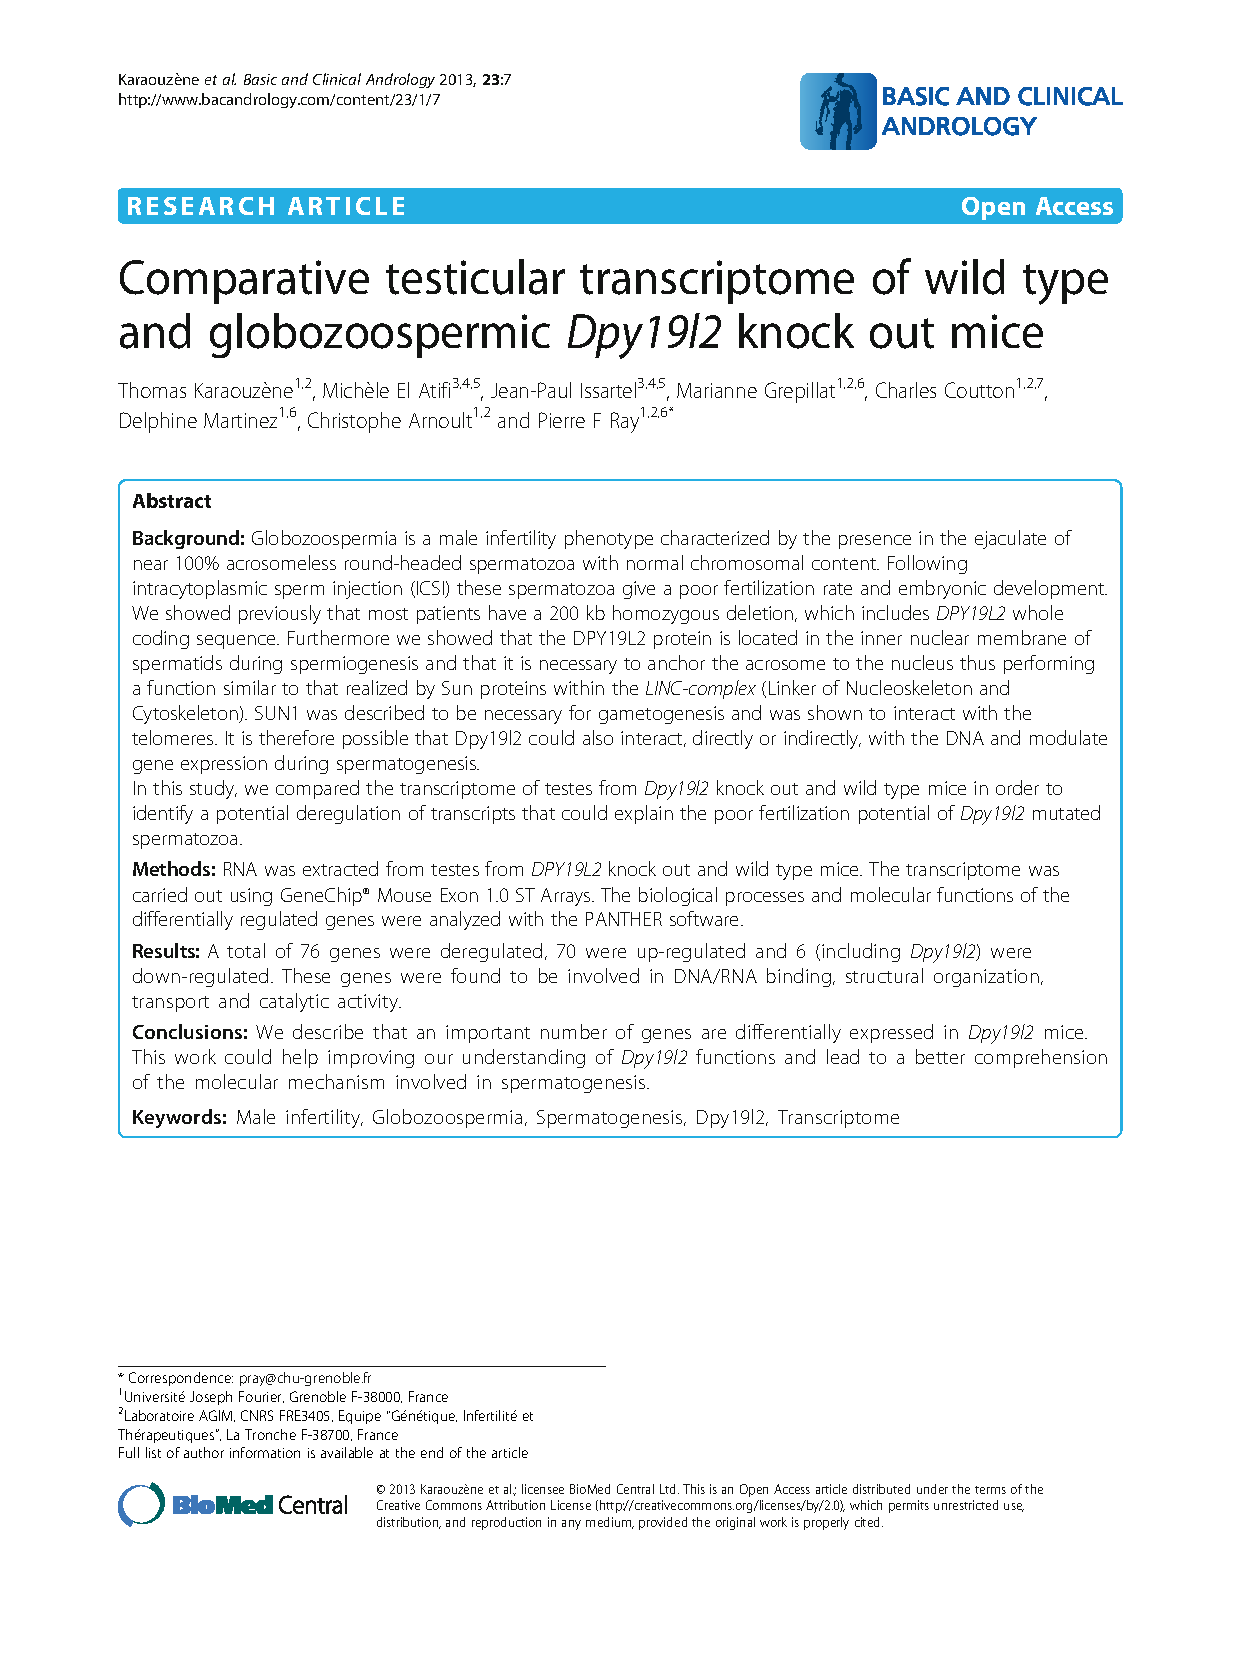
\includepdf[pages=-]{bib/12610_2013_Article_8.pdf}

\newpage

\subsubsection{Principaux résultats :}\label{principaux-resultats-1}

Pour effectuer ces analyses, nous avons donc extrait l'ARN testiculaire
des 4 souris que nous avons ensuite hybridé sur des puces à ADN
Affymetrix GeneChip® Mouse Exon 1.0 contenant des sondes pour 35.557
gènes murins. Cette étape nous a alors permis d'obtenir pour chacune des
4 souris les valeurs d'expression testiculaire de l'ensemble de leurs
gènes. Pour chacun de ces gènes, nous avons donc chercher à savoir s'ils
étaient différentiellement exprimés chez les souris
S1\textsuperscript{-} et S2\textsuperscript{-} lorsqu'on comparait leur
expression avec celle des souris S1\textsuperscript{+} et
S2\textsuperscript{+}. Pour cela, nous avons calculé quatre ratios (R1,
R2, R3 et R4) (\textbf{Équation} : \eqref{eq:micerate}). Les gènes pour
lesquels au moins 3 de leurs ratios étaient \(\ge\) 1,7 furent
considérés comme sur-exprimés tandis que ceux pour lesquels 3 de leurs
ratio étaient \(\le\) 0,58 (\(\frac{1}{1,7}\)) furent considérés comme
sous-exprimés.\\

\begin{equation} 
\begin{split}
\forall gene \in & \ \{genes\ in\ array\}: \\
\\
& R1_{gene} = \frac{exp_{gene}(S1^-)}{exp_{gene}(S1^+)} \ \ \ \ R2_{gene} = \frac{exp_{gene}(S2^-)}{exp_{gene}(S1^+)} \\
& R3_{gene} = \frac{exp_{gene}(S1^-)}{exp_{gene}(S2^+)} \ \ \ \ R4_{gene} = \frac{exp_{gene}(S2^-)}{exp_{gene}(S2^+)} 
\label{eq:micerate}
\end{split}
\end{equation}

De cette manière cette étude a pu mettre en évidence la sous-expression
de 6 gènes (incluant \emph{Dpy19l2}) et la sur-expression de 70 gènes
chez les souris \emph{Dpy19l2}\(^{-/-}\). Parmi ces gènes, nous ne
figurait pas \emph{Plc}\(\zeta\) indiquant que l'absence de cette
protéine chez les spermatozoïdes globozoocéphales n'étaient pas
directement due à un dysfonctionnement transcriptionnel. Afin de prédire
les fonctions moléculaires dans lesquels étaient impliqués ces gènes,
nous nous sommes servis du logiciel PANTHER
{[}\protect\hyperlink{ref-Mi2017}{24}{]}. Ainsi, nous avons pu constater
que 23 gènes codant pour des protéines de liaison étaient dérégulés
(\textbf{Figure : }\ref{fig:plotmolfunction} - \textbf{A}), dont sont
des protéines de liaison aux acides nucléiques (\textbf{Figure :
}\ref{fig:plotmolfunction} - \textbf{B}) suggérant que \emph{Dpy19l2}
pourrait effectivement interagir avec l'ADN. D'autre fonctions
moléculaires telles que l'activité catalytique, la régulation de la
transcription et des protéines ayant des fonctions structurelles étaient
également dérégulées chez les souris KO. Ces derniers sont
particulièrement intéressant lorsque l'on sait que les spermatozoïdes
globozoocéphales sont caractérisés par plusieurs défauts structurels.

Cette étude a pour nous été l'occasion de mieux caractériser la protéine
\emph{Dpy19l2} chez la souris. Nous avons ainsi pu montrer que les
souris \emph{Dpy19l2}\(^{-/-}\) présentaient des dérèglements
transcriptionnels affectant plusieurs fonctions moléculaires pouvant
ainsi expliquer, du moins en partie, les nombreux défauts morphologiques
caractérisant les spermatozoïdes globozoocéphales. De même, nous avons
pu observer le dérèglement de nombreux gènes impliqués dans la liaison
d'acide nucléique et de protéine pouvant ainsi expliquer les défauts
d'ancrage de l'acrosome au noyau chez les spermatozoïdes
globozoocéphales.

Ces résultats ne nous ont cependant pas permis d'expliquer l'absence de
la protéine Plc\(\zeta\) dans le spermatozoïde globocéphale murin
l'expression du gène \emph{Plc}\(\zeta\) n'ayant montré aucune
dérégulation chez la souris \emph{Dpy19l2}\textsuperscript{-/-}. De
même, aucun des gènes retrouvés comme dérégulé ne nous a permis
d'expliquer le biais de sexe que nous avions observés. Cela n'a pas été
une surprise pour nous puisque après avoir entamé notre étude, une
dernière portée issues d'un croisement de souris
\emph{Dpy19l2}\textsuperscript{+/-} a vus le jours. Celle-ci état
composée de 4 souriceaux mâles et de 4 souriceaux femelles. Ainsi, avec
un total de 32 souris mâles pour 20 souris femelles, la p-valeur de
notre test du \(\chi^2\) à 0.0635765 laissant cette fois-ci supposer la
non-existence d'un biais de sexe dans les naissances issues d'un
croisement de souris \emph{Dpy19l2}\textsuperscript{-/-}.

\newpage 

\begin{figure}

{\centering \includegraphics{thesis_files/figure-latex/plotmolfunction-1} 

}

\caption[Principales fonctions moléculaires affectées chez les souris *Dpy19l2* KO]{\textbf{\emph{Principales fonctions moléculaires
affectées chez les souris \emph{Dpy19l2} KO}.} : \textbf{A} : Liste des
fonctions moléculaires affectées : Bndn = Binding, Ctly = Catalytic,
Trnsc = Transcription, Strm = Structural molecule, Rcpt = Receptor.
\textbf{B} : Détails des fonctions moléculaires affectées par les gènes
dérégulés}\label{fig:plotmolfunction}
\end{figure}








\chapter{Mise en place d'une stratégie pour l'analyse des données
exomiques -- application en recherche
clinique}\label{mise-en-place-dune-strategie-pour-lanalyse-des-donnees-exomiques-application-en-recherche-clinique}

\chapter*{Conclusion et discussion}\label{conclusion-et-discussion}
\addcontentsline{toc}{chapter}{Conclusion et discussion}

\chapter{Mutations in DNAH1, which Encodes an Inner Arm Heavy Chain
Dynein, Lead to Male Infertility from Multiple Morphological
Abnormalities of the Sperm Flagella}\label{dnah12014}

\chapter*{References}\label{references}
\addcontentsline{toc}{chapter}{References}

\hypertarget{refs}{}
\hypertarget{ref-Sen2009}{}
1. C.G.S. Sen, A.F. Holstein, and C. Schirren: ``über die Morphogenese
rundköpfiger Spermatozoen des Menschen.'' \emph{Andrologia}. vol. 3, no.
3, pp. 117--125, 1971.

\hypertarget{ref-Singh}{}
2. G. Singh: ``Ultrastructural features of round-headed human
spermatozoa.'' \emph{International journal of fertility}. vol. 37, no.
2, pp. 99--102,

\hypertarget{ref-Pedersen1974}{}
3. H. Pedersen and H. Rebbe: ``Fine structure of round-headed human
spermatozoa.'' \emph{Journal of reproduction and fertility}. vol. 37,
no. 1, pp. 51--4, 1974.

\hypertarget{ref-Heytens2009}{}
4. E. Heytens, J. Parrington, K. Coward, C. Young, S. Lambrecht, S.-Y.
Yoon, R.A. Fissore, R. Hamer, C.M. Deane, M. Ruas, P. Grasa, R.
Soleimani, C.A. Cuvelier, J. Gerris, M. Dhont, D. Deforce, L. Leybaert,
and P. De Sutter: ``Reduced amounts and abnormal forms of phospholipase
C zeta (PLCzeta) in spermatozoa from infertile men.'' \emph{Human
reproduction (Oxford, England)}. vol. 24, no. 10, pp. 2417--28, 2009.

\hypertarget{ref-Taylor2010}{}
5. S. Taylor, S. Yoon, M. Morshedi, D. Lacey, T. Jellerette, R. Fissore,
and S. Oehninger: ``Complete globozoospermia associated with
PLC\(\zeta\) deficiency treated with calcium ionophore and ICSI results
in pregnancy.'' \emph{Reproductive BioMedicine Online}. vol. 20, no. 4,
pp. 559--564, 2010.

\hypertarget{ref-Yoon2008}{}
6. S.-Y. Yoon, T. Jellerette, A.M. Salicioni, H.C. Lee, M.-S. Yoo, K.
Coward, J. Parrington, D. Grow, J.B. Cibelli, P.E. Visconti, J. Mager,
and R.A. Fissore: ``Human sperm devoid of PLC, zeta 1 fail to induce
Ca(2+) release and are unable to initiate the first step of embryo
development.'' \emph{The Journal of clinical investigation}. vol. 118,
no. 11, pp. 3671--81, 2008.

\hypertarget{ref-Dam2006}{}
7. A. Dam, I. Feenstra, J. Westphal, L. Ramos, R. van Golde, and J.
Kremer: ``Globozoospermia revisited.'' \emph{Human Reproduction Update}.
vol. 13, no. 1, pp. 63--75, 2006.

\hypertarget{ref-Dam2007}{}
8. A.H.D.M. Dam, I. Koscinski, J.A.M. Kremer, C. Moutou, A.-S. Jaeger,
A.R. Oudakker, H. Tournaye, N. Charlet, C. Lagier-Tourenne, H. van
Bokhoven, and S. Viville: ``Homozygous mutation in SPATA16 is associated
with male infertility in human globozoospermia.'' \emph{American journal
of human genetics}. vol. 81, no. 4, pp. 813--20, 2007.

\hypertarget{ref-Harbuz2011}{}
9. R. Harbuz, R. Zouari, V. Pierre, M. Ben Khelifa, M. Kharouf, C.
Coutton, G. Merdassi, F. Abada, J. Escoffier, Y. Nikas, F. Vialard, I.
Koscinski, C. Triki, N. Sermondade, T. Schweitzer, A. Zhioua, F. Zhioua,
H. Latrous, L. Halouani, M. Ouafi, M. Makni, P.-S. Jouk, B. Sèle, S.
Hennebicq, V. Satre, S. Viville, C. Arnoult, J. Lunardi, and P.F. Ray:
``A recurrent deletion of DPY19L2 causes infertility in man by blocking
sperm head elongation and acrosome formation.'' \emph{American journal
of human genetics}. vol. 88, no. 3, pp. 351--61, 2011.

\hypertarget{ref-Ray2011}{}
10. P.F. Ray and C. Arnoult: ``La délétion homozygote du gène
\textless{}i\textgreater{}DPY19L2\textless{}/i\textgreater{} est
responsable de la majorité des cas de globozoospermie.''
\emph{médecine/sciences}. vol. 27, no. 8-9, pp. 692--693, 2011.

\hypertarget{ref-ElInati2012}{}
11. E. ElInati, P. Kuentz, C. Redin, S. Jaber, F. Vanden Meerschaut, J.
Makarian, I. Koscinski, M.H. Nasr-Esfahani, A. Demirol, T. Gurgan, N.
Louanjli, N. Iqbal, M. Bisharah, F.C. Pigeon, H. Gourabi, D. De Briel,
F. Brugnon, S.A. Gitlin, J.-M. Grillo, K. Ghaedi, M.R. Deemeh, S.
Tanhaei, P. Modarres, B. Heindryckx, M. Benkhalifa, D. Nikiforaki, S.C.
Oehninger, P. De Sutter, J. Muller, and S. Viville: ``Globozoospermia is
mainly due to DPY19L2 deletion via non-allelic homologous recombination
involving two recombination hotspots.'' \emph{Human Molecular Genetics}.
vol. 21, no. 16, pp. 3695--3702, 2012.

\hypertarget{ref-Pierre2012}{}
12. V. Pierre, G. Martinez, C. Coutton, J. Delaroche, S. Yassine, C.
Novella, K. Pernet-Gallay, S. Hennebicq, P.F. Ray, and C. Arnoult:
``Absence of Dpy19l2, a new inner nuclear membrane protein, causes
globozoospermia in mice by preventing the anchoring of the acrosome to
the nucleus.'' \emph{Development}. vol. 139, no. 16, pp. 2955--2965,
2012.

\hypertarget{ref-Carson2006}{}
13. A.R. Carson, J. Cheung, and S.W. Scherer: ``Duplication and
relocation of the functional DPY19L2 gene within low copy repeats.''
\emph{BMC genomics}. vol. 7, pp. 45, 2006.

\hypertarget{ref-Cheung2003}{}
14. J. Cheung, X. Estivill, R. Khaja, J.R. MacDonald, K. Lau, L.-C.
Tsui, and S.W. Scherer: ``Genome-wide detection of segmental
duplications and potential assembly errors in the human genome
sequence.'' \emph{Genome biology}. vol. 4, no. 4, pp. R25, 2003.

\hypertarget{ref-Bailey2002}{}
15. J.A. Bailey, Z. Gu, R.A. Clark, K. Reinert, R.V. Samonte, S.
Schwartz, M.D. Adams, E.W. Myers, P.W. Li, and E.E. Eichler: ``Recent
Segmental Duplications in the Human Genome.'' \emph{Science}. vol. 297,
no. 5583, pp. 1003--1007, 2002.

\hypertarget{ref-Walsh2003}{}
16. B. Walsh: ``Population-genetic models of the fates of duplicate
genes.'' \emph{Genetica}. vol. 118, no. 2-3, pp. 279--94, 2003.

\hypertarget{ref-Ohno1970}{}
17. S. Ohno: ``Evolution by Gene Duplication.'' \emph{Springer Berlin
Heidelberg}, Berlin, Heidelberg, 1970.

\hypertarget{ref-Harbuz2011a}{}
18. R. Harbuz, R. Zouari, V. Pierre, M. Ben Khelifa, M. Kharouf, C.
Coutton, G. Merdassi, F. Abada, J. Escoffier, Y. Nikas, F. Vialard, I.
Koscinski, C. Triki, N. Sermondade, T. Schweitzer, A. Zhioua, F. Zhioua,
H. Latrous, L. Halouani, M. Ouafi, M. Makni, P.-S. Jouk, B. Sèle, S.
Hennebicq, V. Satre, S. Viville, C. Arnoult, J. Lunardi, and P.F. Ray:
``A recurrent deletion of DPY19L2 causes infertility in man by blocking
sperm head elongation and acrosome formation.'' \emph{American journal
of human genetics}. vol. 88, no. 3, pp. 351--61, 2011.

\hypertarget{ref-Liu2012}{}
19. P. Liu, C.M. Carvalho, P. Hastings, and J.R. Lupski: ``Mechanisms
for recurrent and complex human genomic rearrangements.'' \emph{Current
Opinion in Genetics \& Development}. vol. 22, no. 3, pp. 211--220, 2012.

\hypertarget{ref-MacDonald2014}{}
20. J.R. MacDonald, R. Ziman, R.K.C. Yuen, L. Feuk, and S.W. Scherer:
``The Database of Genomic Variants: a curated collection of structural
variation in the human genome.'' \emph{Nucleic acids research}. vol. 42,
no. Database issue, pp. D986--92, 2014.

\hypertarget{ref-Parvanov2010}{}
21. E.D. Parvanov, P.M. Petkov, and K. Paigen: ``Prdm9 controls
activation of mammalian recombination hotspots.'' \emph{Science (New
York, N.Y.)}. vol. 327, no. 5967, pp. 835, 2010.

\hypertarget{ref-Baudat2010}{}
22. F. Baudat, J. Buard, C. Grey, A. Fledel-Alon, C. Ober, M.
Przeworski, G. Coop, and B. de Massy: ``PRDM9 is a major determinant of
meiotic recombination hotspots in humans and mice.'' \emph{Science (New
York, N.Y.)}. vol. 327, no. 5967, pp. 836--40, 2010.

\hypertarget{ref-Ding2007}{}
23. X. Ding, R. Xu, J. Yu, T. Xu, Y. Zhuang, and M. Han: ``SUN1 Is
Required for Telomere Attachment to Nuclear Envelope and Gametogenesis
in Mice.'' \emph{Developmental Cell}. vol. 12, no. 6, pp. 863--872,
2007.

\hypertarget{ref-Mi2017}{}
24. H. Mi, X. Huang, A. Muruganujan, H. Tang, C. Mills, D. Kang, and
P.D. Thomas: ``PANTHER version 11: expanded annotation data from Gene
Ontology and Reactome pathways, and data analysis tool enhancements.''
\emph{Nucleic Acids Research}. vol. 45, no. D1, pp. D183--D189, 2017.


% Index?

\end{document}

